\documentclass[11pt]{article}
\usepackage{color,amsmath,amsfonts,amssymb,amsthm}

\usepackage[pdftex]{graphicx}
\DeclareGraphicsExtensions{.pdf, .jpg, .tif, .png}
\usepackage{rotating}

\textwidth=7.0in
\textheight=8.75in
\topmargin=-0.5in
\headsep=0.0in
\headheight=0.5in
\oddsidemargin=-0.25in
\evensidemargin=-0.25in

\usepackage{array}
\newcolumntype{L}[1]{>{\raggedright\let\newline\\\arraybackslash\hspace{0pt}}m{#1}}
\newcolumntype{C}[1]{>{\centering\let\newline\\\arraybackslash\hspace{0pt}}m{#1}}
\newcolumntype{R}[1]{>{\raggedleft\let\newline\\\arraybackslash\hspace{0pt}}m{#1}}

\begin{document}
{\bf Proposed repository workflow for MPAS cores within LANL.}\\
December 12, 2014\\
Mark Petersen\\

{\bf Requirements}
\begin{enumerate}
\item Upon completion, a new feature may be labeled as releasable or private.
\item Releasable features will be available to the public in the next release that the core participates in.
\item Private features will be available on the private branch, which is for LANL use only.
\item A development branch will be provided, which includes all releasable features.  
\item The development branch must be ready to release at any time.
\item A private branch will be provided for simulations internal to LANL, which includes both private and releasable features.
\item When private features are deemed releasable, they may be added to the development branch.
\item The private branch will occasionally be synchronized with the development branch, so that the private branch does not drift too far.  Ideally, the private branch is identical to the development branch, but with all private features added in.
\item Simulations for publications should be conducted on a permanent hash (a state the will be in the repository indefinitely).  We can't require this, but the the functionality should be there in the repository.
\item ACME can only point to a permanent hash.
\item The ability to release one feature should not depend on the private/releasable status of any other feature.
\item The ACME repository can only point to an MPAS-Core hash that can be public when ACME is eventually released.
\item ACME may be changed locally to point to other MPAS-core hashes.  These must be permanent hashes, and may be future-releasable or forever-private branches.
\end{enumerate}

\clearpage

{\bf Definitions:}\\

Developer: designs, codes, and tests new features.  Responsible for their own feature branches.

Maintainer: developer, plus responsible for shared branches (release, development, and private branches)\\

{\bf Branches:}
\begin{enumerate}
\item \verb| MPAS_Dev/develop|  Framework development branch and release branch.  Framework-level changes are branched from and merged back into here.   All commits to this branch are releasable.  Public releases are tagged from this branch.

\item \verb| MPAS_Dev/core/develop|  Core development branch.  Core-level changes are branched from and merged back into here.  All commits to this branch are releasable.

\item \verb| MPAS_Dev/core/private_v*|  Internal LANL branch.  This ideally is the core/develop branch with completed private features added in, but the branch will sometimes lag behind core/develop.  These branches are permanent, and are intended for simulations within LANL where private features are needed.

\item \verb| core/feature_branch|  Feature development branch, private to the developer, and on his/her fork.  These are not permanent, and are intended for eventual merger into the development or private branch after completion.
\end{enumerate}

{\bf Workflow:}

\begin{enumerate}
\item Start a new feature

 \begin{tabular}[c]{L{3.25in}|L{3.25in}}
developer & maintainer \\
\hline
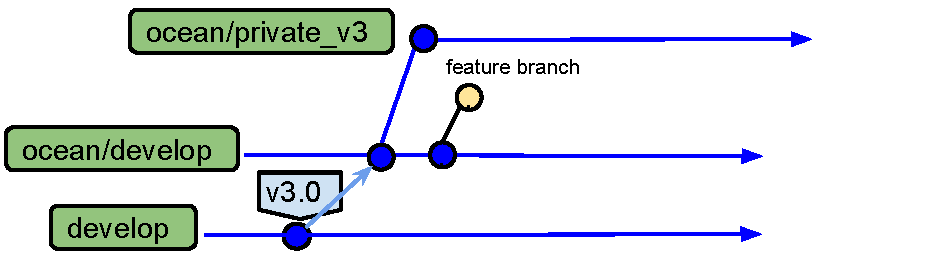
\includegraphics[width=3.25in]{f/MPASworkflow_1.pdf} \\
\\
\verb| git checkout MPAS-Dev/ocean/develop | \\
\verb| git branch --no-track my_branch|  \\
\verb| git push my_fork my_branch|  & 
 \end{tabular}
\item Commit changes to feature 

 \begin{tabular}[c]{L{3.25in}|L{3.25in}}
developer & maintainer \\
\hline
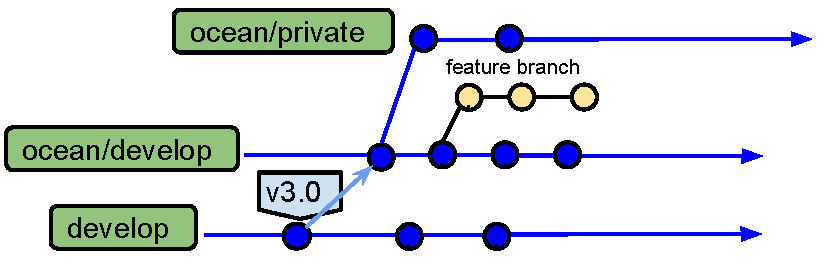
\includegraphics[width=3.25in]{f/MPASworkflow_2.pdf} \\
\verb| git commit -a|  \\
\verb| git push my_fork my_branch|  
 \end{tabular}

\clearpage
\item Completion of releasable feature

\begin{centering}
\end{centering}
 \begin{tabular}[c]{L{3.25in}|L{3.25in}}
developer & maintainer \\
\hline
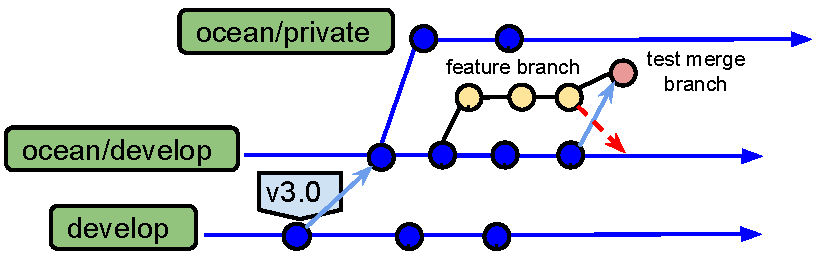
\includegraphics[width=3.25in]{f/MPASworkflow_3d.pdf} & 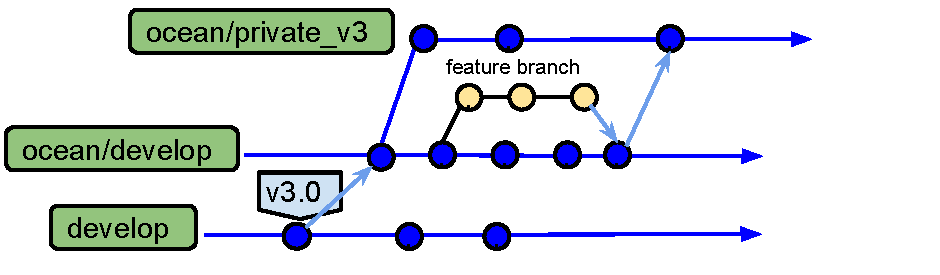
\includegraphics[width=3.25in]{f/MPASworkflow_3.pdf} \\
All development and testing must be complete.
Create a test merge branch: \\
\verb| git branch --no-track test_merge|  \\
\verb| git merge MPAS-Dev/ocean/develop|  \\
Test, resolve conflicts \\
\verb| git commit -a|  \\
\verb| git push my_fork test_merge| \\
Create pull request from \verb|my_branch| to \verb|MPAS-Dev/ocean/develop| at github.com \\
& merge feature branch onto ocean/develop \\
& merge ocean/develop onto ocean/private\_v* (if desired)\\
delete local and remote feature branches: \\
\verb| git branch -D my_branch|  \\
\verb| git branch -D test_merge|  \\
\verb| git push my_fork :my_branch| \\
\verb| git push my_fork :test_merge| \\
 \end{tabular}

\clearpage
\item Completion of private feature

\begin{centering}
\end{centering}
 \begin{tabular}[c]{L{3.25in}|L{3.25in}}
developer & maintainer \\
\hline
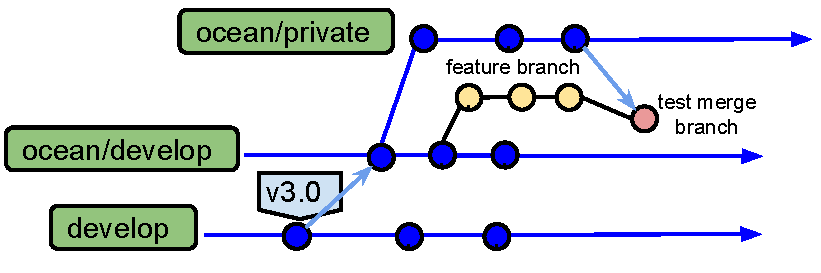
\includegraphics[width=3.25in]{f/MPASworkflow_4d.pdf} & 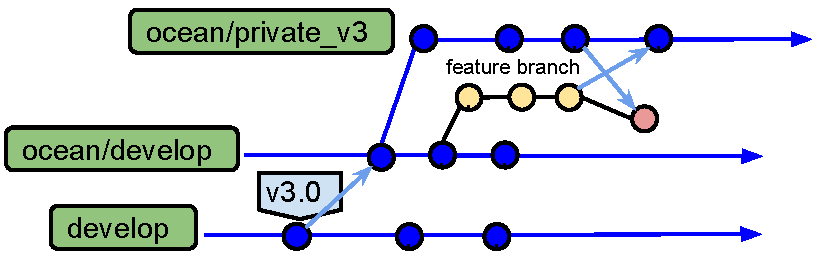
\includegraphics[width=3.25in]{f/MPASworkflow_4.pdf} \\
All development and testing must be complete.
Create a test merge branch: \\
\verb| git branch --no-track test_merge|  \\
\verb| git merge MPAS-Dev/ocean/private_v*|  \\
Test, resolve conflicts \\
\verb| git commit -a|  \\
\verb| git push my_fork test_merge| \\
Create pull request from \verb|my_branch| to both \verb|MPAS-Dev/ocean/develop| and \verb|MPAS-Dev/ocean/private_v*| at github.com. \\
& merge feature branch onto ocean/private\_v* \\
delete local and remote test branches: \\
\verb| git branch -D test_merge|  \\
\verb| git push my_fork :test_merge| \\
 \end{tabular}

Note that for a private feature, the feature branch is not deleted, and the pull request to ocean/develop remains open.  This is a way to track completed private features, which are not on ocean/develop.

\item Alterations of releasable feature after completion\\
Treat this as a new feature or bug fix, follow steps 1--3.

\item Alterations of private feature after completion\\
Commit additional changes to feature branch per step 2, then merge to the private branch per step 4.  If ocean/develop has changed substantially, the developer may prefer to rebase the feature branch on ocean/develop, or just completely recreate it, repeating step 1 and deleting the old feature branch.

\item Feature changes from private to releasable \\
Merge feature onto ocean/develop per step 3.  Again, if ocean/develop has changed substantially, the developer may prefer to rebase the feature branch on ocean/develop, or just completely recreate it, repeating step 1 and deleting the old feature branch.

\item Keep private branch synchronized with development branch.

Method 1: Merge ocean/develop onto ocean/private\_v*.  This may be done when new features on ocean/develop are needed on ocean/private\_v*, as in step 3 above.

Method 2: Create new ocean/private\_v*, and then merge in all completed private features.  This will be done rarely, like once every release cycle or less, but is important for compatibility of private feature branches between ocean/develop and ocean/private\_v*.  Maintainers create the new branch, but developers are responsibile for updating their private feature branches to the new version, if desired, essentially repeating step 4 above.

All ocean/private\_v* branches are kept permanently on a private branch at \verb|MPAS-Dev|, and are available to all LANL users.  LANL users and developers may remain on an older version of ocean/private\_v* to complete particular projects, if desired.

\end{enumerate}





% \begin{figure}[btp]
% \centering
% \begin{tabular}[c]{cccc}
% & tracer & layerThickness & maxLevelCell \\
% \begin{sideways}\hspace{0.2in}  bottom layer \end{sideways}&
% \includegraphics[height=1.5in, clip,trim=0 0 0 0]{f/c24u/c24u_DOME_temperature_b_20days_zoom.pdf} &
% \includegraphics[height=1.5in, clip,trim=0 0  0 0]{f/c24u/c24u_DOME_avgLayerThickness_b_20days_zoom.pdf}&
% \includegraphics[height=1.5in, clip,trim=0 0  0 0]{f/c24u/c24u_DOME_maxLevelCell_2_20days_zoom.pdf}\\
% \begin{sideways}\hspace{0.2in}  bottom layer-1 \end{sideways}&
% \includegraphics[height=1.5in, clip,trim=0 0 0 0]{f/c24u/c24u_DOME_temperature_B_20days_zoom.pdf} &
% \end{tabular}
% \caption{\label{fig:T striping zoom}
% {\bf 20 days instantaneous} DOME overflow cases, 15m layers, PBCs, zoom on striping.
% }
% \end{figure}

\end{document}


